%----------------------------------------------------------------------------------------

\begin{frame}
\frametitle{
\includegraphics[scale=0.4]{./materials/Genma.jpg} \ \ \  About me }
\begin{columns}[c] 

\column{.55\textwidth} 
\textbf{Where can you find me on Internet?}
\begin{itemize}
\item Blog (in French) : http://genma.free.fr
\item Twitter : http://twitter.com/genma
\end{itemize}

\textbf{My Hobbies? Many things}
\begin{itemize}
\item Crypto
\item Privacy
\end{itemize}

\column{.5\textwidth} 
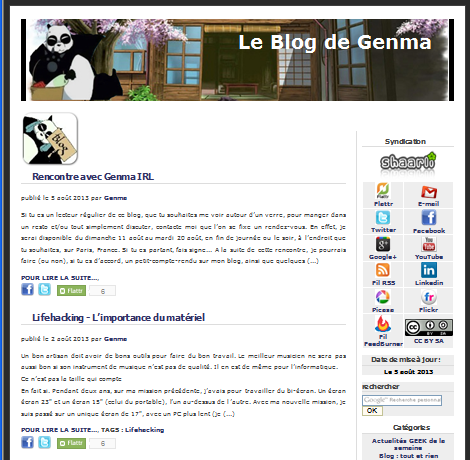
\includegraphics[width=5cm,height=5cm]{./materials/blog.png} 
\end{columns}
\end{frame}


%----------------------------------------------------------------------------------------
\begin{frame}
\frametitle{Digital identity, what is it?}


\begin{block}{Definition}
\begin{itemize}
\justifying{
\item Digital identity is all the public data you can find about someone using Internet research.
\item It's the famous e-reputation.
}
\end{itemize}
\end{block}
\end{frame}

%----------------------------------------------------------------------------------------
\begin{frame}
\frametitle{What do you think of me?}

\justifying{
\begin{block}{Google you name}
\begin{itemize}
\item The results shown are they exactly what you want?
\end{itemize}
\end{block}
}
\begin{center}
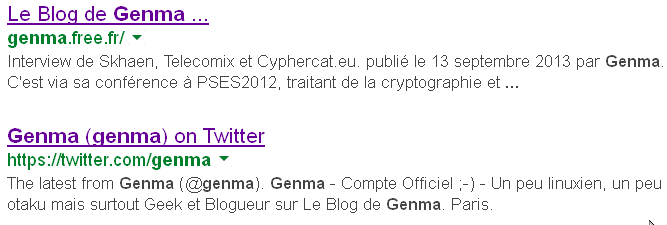
\includegraphics[scale=0.3] {./materials/Google01.png}
\\
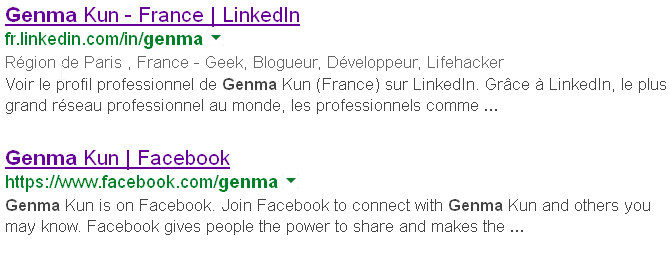
\includegraphics[scale=0.3] {./materials/Google02.png}
\end{center}
\end{frame}

%----------------------------------------------------------------------------------------
\begin{frame}
\frametitle{Saying}

\begin{block}{Words fly, writings remain}
\begin{itemize}
\justifying{
\item This adage is especially true with the Internet.
\item It must be assumed that what is said will always be accessible, even years later.
\item Everything on the Internet is public or will be (even if it is "private", Terms of Use may change).
\item It is therefore not abuse the freedom of expression and remain respectful of laws.
}
\end{itemize}
\end{block}


\end{frame}

%----------------------------------------------------------------------------------------
\begin{frame}
\frametitle{Pseudonymity}


\begin{block}{Defintion}
\begin{itemize}
\justifying{
\item Contraction of anonymity and pseudonym words, the term pseudonymity reflects quite well the contradictory of \textbf{being a public figure and to remain anonymous} ...
\item Have a pseudonym does not mean to say and do anything.
\item This is the image that I return, this is my credibility (past, present and future).
\item A pseudonym is also a public identity, which is associated with different account: my blog, my Twitter, my Facebook account.
\item The digital identity are all these public data associated with this identity.
}
\end{itemize}
\end{block}

\end{frame}


%----------------------------------------------------------------------------------------
\begin{frame}
\frametitle{Samples}

\begin{block}{Twitter}
\begin{center}
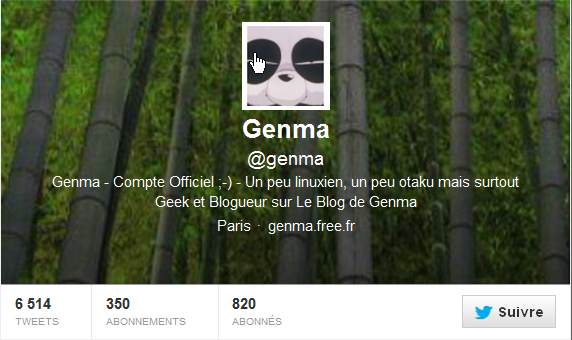
\includegraphics[scale=0.2] {./materials/Twitter.png}
\end{center}
\end{block}

\begin{block}{Linkedin}
\begin{center}
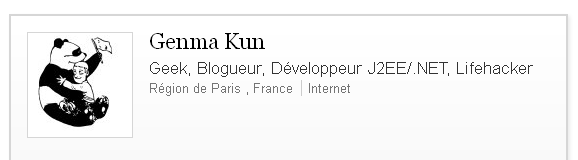
\includegraphics[scale=0.3] {./materials/Linkedin.png}
\end{center}
\end{block}
\end{frame}


%----------------------------------------------------------------------------------------
\begin{frame}
\frametitle{Pseudonymity is disapearing...}

\justifying{
\begin{block}{Facebook}
\begin{itemize}
\item Facebook doesn't allow an account with a pseudonym.
\item O RLY? Look \url{http://www.facebook.com/genma} ;-)
\end{itemize}
\end{block}
}

\justifying{
\begin{block}{Pseudonymity is a necessity}
\begin{itemize}
\item Manage your digital identity.
\item \textbf{Pseudonymity is the first step to take back you privacy.}
\end{itemize}
\end{block}
}

\end{frame}

